\documentclass[a4paper]{report}


\usepackage[T1]{fontenc} % codifica dei font per l'italiano
\usepackage[utf8]{inputenc} % lettere accentate da tastiera
\usepackage[italian]{babel} % lingua del documento
\usepackage[shortlabels]{enumitem}%per fare elenchi ad hoc
\usepackage{framed}% per riquadrare il testo
\usepackage{amsmath}% per avere le formule matematiche fatte bene
\usepackage{amssymb}% per avere le formule matematiche fatte bene
\usepackage{amsthm}%per fare i teoremi in modo ordinato
\usepackage[big]{layaureo} %per avere i margini più stretti
\usepackage{graphicx} %per inserire le immagini
\usepackage{mathtools}
\usepackage{mathabx}

%immagini
\usepackage{amsmath}
\usepackage{tikz}
\usepackage{mathdots}
\usepackage{yhmath}
\usepackage{cancel}
\usepackage{color}
\usepackage{siunitx}
\usepackage{array}
\usepackage{multirow}
\usepackage{amssymb}
\usepackage{gensymb}
\usepackage{tabularx}
\usepackage{booktabs}
\usetikzlibrary{fadings}
\usetikzlibrary{patterns}
\usetikzlibrary{shadows.blur}
\usetikzlibrary{shapes}

\makeatletter
\newcommand{\superimpose}[2]{%
  {\ooalign{$#1\@firstoftwo#2$\cr\hfil$#1\@secondoftwo#2$\hfil\cr}}}
\makeatother
\def\retro{\ensuremath{%
  \reflectbox{\rotatebox[origin=c]{180}{$\circlearrowleft$}}}}
\newcommand{\R}{\mathbb{R}}%reali
\newcommand{\retroneg}{\mathpalette\superimpose{{\retro}{-}}} %retroazione negativa
\DeclareMathOperator{\tr}{tr} %traccia
\newcommand{\parallelsum}{\mathbin{\|}}%parallelo

\graphicspath{ {./images/} }


\begin{document}
\begin{center}

\section*{Risoluzione Esercizi di Simulazione}
Luca Maci e Jacopo Stringara
\end{center}
\subsection*{Quesito 1}
\begin{figure}[h]
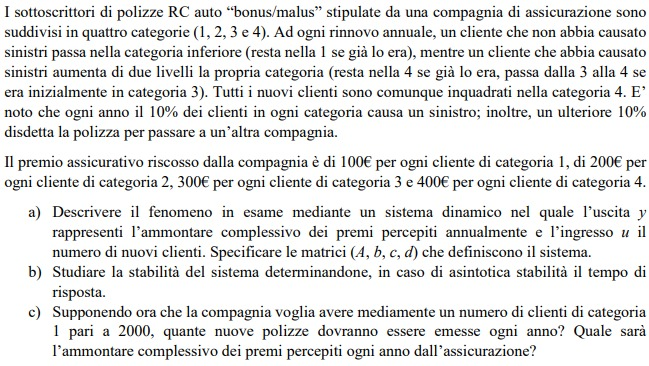
\includegraphics[width=\textwidth]{prima_domanda}
\end{figure}
\underline{Risposte:}
\begin{enumerate}[a)]
\item Leggendo il testo del problema ci è facile disegnare il modello seguente:




\tikzset{every picture/.style={line width=0.75pt}} %set default line width to 0.75pt        

\begin{tikzpicture}[x=0.75pt,y=0.75pt,yscale=-1,xscale=1]
%uncomment if require: \path (0,300); %set diagram left start at 0, and has height of 300

%Shape: Circle [id:dp5022504860822765] 
\draw   (95,126.25) .. controls (95,112.44) and (106.19,101.25) .. (120,101.25) .. controls (133.81,101.25) and (145,112.44) .. (145,126.25) .. controls (145,140.06) and (133.81,151.25) .. (120,151.25) .. controls (106.19,151.25) and (95,140.06) .. (95,126.25) -- cycle ;

%Shape: Circle [id:dp5803418704093459] 
\draw   (491,126.25) .. controls (491,112.44) and (502.19,101.25) .. (516,101.25) .. controls (529.81,101.25) and (541,112.44) .. (541,126.25) .. controls (541,140.06) and (529.81,151.25) .. (516,151.25) .. controls (502.19,151.25) and (491,140.06) .. (491,126.25) -- cycle ;

%Shape: Circle [id:dp01920206383687817] 
\draw   (359,126.25) .. controls (359,112.44) and (370.19,101.25) .. (384,101.25) .. controls (397.81,101.25) and (409,112.44) .. (409,126.25) .. controls (409,140.06) and (397.81,151.25) .. (384,151.25) .. controls (370.19,151.25) and (359,140.06) .. (359,126.25) -- cycle ;

%Shape: Circle [id:dp8268925753397789] 
\draw   (227,126.25) .. controls (227,112.44) and (238.19,101.25) .. (252,101.25) .. controls (265.81,101.25) and (277,112.44) .. (277,126.25) .. controls (277,140.06) and (265.81,151.25) .. (252,151.25) .. controls (238.19,151.25) and (227,140.06) .. (227,126.25) -- cycle ;

%Straight Lines [id:da83309083141393] 
\draw    (359,126.25) -- (279,126.25) ;
\draw [shift={(277,126.25)}, rotate = 360] [color={rgb, 255:red, 0; green, 0; blue, 0 }  ][line width=0.75]    (10.93,-3.29) .. controls (6.95,-1.4) and (3.31,-0.3) .. (0,0) .. controls (3.31,0.3) and (6.95,1.4) .. (10.93,3.29)   ;
%Straight Lines [id:da39632635329626464] 
\draw    (491,126.25) -- (411,126.25) ;
\draw [shift={(409,126.25)}, rotate = 360] [color={rgb, 255:red, 0; green, 0; blue, 0 }  ][line width=0.75]    (10.93,-3.29) .. controls (6.95,-1.4) and (3.31,-0.3) .. (0,0) .. controls (3.31,0.3) and (6.95,1.4) .. (10.93,3.29)   ;
%Straight Lines [id:da015987837758611123] 
\draw    (227,126.25) -- (147,126.25) ;
\draw [shift={(145,126.25)}, rotate = 360] [color={rgb, 255:red, 0; green, 0; blue, 0 }  ][line width=0.75]    (10.93,-3.29) .. controls (6.95,-1.4) and (3.31,-0.3) .. (0,0) .. controls (3.31,0.3) and (6.95,1.4) .. (10.93,3.29)   ;

%Curve Lines [id:da4921395161805495] 
\draw    (120,101.25) .. controls (131.44,57.22) and (357.23,27.3) .. (383.62,100.14) ;
\draw [shift={(384,101.25)}, rotate = 251.74] [color={rgb, 255:red, 0; green, 0; blue, 0 }  ][line width=0.75]    (10.93,-3.29) .. controls (6.95,-1.4) and (3.31,-0.3) .. (0,0) .. controls (3.31,0.3) and (6.95,1.4) .. (10.93,3.29)   ;
%Curve Lines [id:da12410751681984111] 
\draw    (252,101.25) .. controls (263.44,57.22) and (489.23,27.3) .. (515.62,100.14) ;
\draw [shift={(516,101.25)}, rotate = 251.74] [color={rgb, 255:red, 0; green, 0; blue, 0 }  ][line width=0.75]    (10.93,-3.29) .. controls (6.95,-1.4) and (3.31,-0.3) .. (0,0) .. controls (3.31,0.3) and (6.95,1.4) .. (10.93,3.29)   ;
%Curve Lines [id:da13031986513998062] 
\draw    (384,101.25) .. controls (423.6,71.55) and (460.26,78.6) .. (503.2,103.25) ;
\draw [shift={(504.5,104)}, rotate = 210.13] [color={rgb, 255:red, 0; green, 0; blue, 0 }  ][line width=0.75]    (10.93,-3.29) .. controls (6.95,-1.4) and (3.31,-0.3) .. (0,0) .. controls (3.31,0.3) and (6.95,1.4) .. (10.93,3.29)   ;
%Curve Lines [id:da5834598691765318] 
\draw    (95.5,121) .. controls (87.5,95) and (36.5,102) .. (37.5,124) .. controls (38.5,146) and (50.57,147.6) .. (62.5,150) .. controls (73.71,152.25) and (85.72,145.09) .. (94.8,139.95) ;
\draw [shift={(96.5,139)}, rotate = 510.95] [color={rgb, 255:red, 0; green, 0; blue, 0 }  ][line width=0.75]    (10.93,-3.29) .. controls (6.95,-1.4) and (3.31,-0.3) .. (0,0) .. controls (3.31,0.3) and (6.95,1.4) .. (10.93,3.29)   ;
%Curve Lines [id:da06725770645640528] 
\draw    (528.5,104) .. controls (520.5,78) and (558.5,64) .. (569.5,78) .. controls (580.39,91.86) and (585.4,110.62) .. (539.89,115.85) ;
\draw [shift={(538.5,116)}, rotate = 353.93] [color={rgb, 255:red, 0; green, 0; blue, 0 }  ][line width=0.75]    (10.93,-3.29) .. controls (6.95,-1.4) and (3.31,-0.3) .. (0,0) .. controls (3.31,0.3) and (6.95,1.4) .. (10.93,3.29)   ;
%Straight Lines [id:da42440620300568943] 
\draw    (602.5,124.38) -- (543,124.62) ;
\draw [shift={(541,124.63)}, rotate = 359.77] [color={rgb, 255:red, 0; green, 0; blue, 0 }  ][line width=0.75]    (10.93,-3.29) .. controls (6.95,-1.4) and (3.31,-0.3) .. (0,0) .. controls (3.31,0.3) and (6.95,1.4) .. (10.93,3.29)   ;
%Straight Lines [id:da8993777412556865] 
\draw    (120,151.25) -- (120.48,200) ;
\draw [shift={(120.5,202)}, rotate = 269.44] [color={rgb, 255:red, 0; green, 0; blue, 0 }  ][line width=0.75]    (10.93,-3.29) .. controls (6.95,-1.4) and (3.31,-0.3) .. (0,0) .. controls (3.31,0.3) and (6.95,1.4) .. (10.93,3.29)   ;
%Straight Lines [id:da6916538293598196] 
\draw    (252,151.25) -- (252.48,200) ;
\draw [shift={(252.5,202)}, rotate = 269.44] [color={rgb, 255:red, 0; green, 0; blue, 0 }  ][line width=0.75]    (10.93,-3.29) .. controls (6.95,-1.4) and (3.31,-0.3) .. (0,0) .. controls (3.31,0.3) and (6.95,1.4) .. (10.93,3.29)   ;
%Straight Lines [id:da35246686482257816] 
\draw    (384,151.25) -- (384.48,200) ;
\draw [shift={(384.5,202)}, rotate = 269.44] [color={rgb, 255:red, 0; green, 0; blue, 0 }  ][line width=0.75]    (10.93,-3.29) .. controls (6.95,-1.4) and (3.31,-0.3) .. (0,0) .. controls (3.31,0.3) and (6.95,1.4) .. (10.93,3.29)   ;
%Straight Lines [id:da12490561774656417] 
\draw    (516,151.25) -- (516.48,200) ;
\draw [shift={(516.5,202)}, rotate = 269.44] [color={rgb, 255:red, 0; green, 0; blue, 0 }  ][line width=0.75]    (10.93,-3.29) .. controls (6.95,-1.4) and (3.31,-0.3) .. (0,0) .. controls (3.31,0.3) and (6.95,1.4) .. (10.93,3.29)   ;

% Text Node
\draw (111,117.65) node [anchor=north west][inner sep=0.75pt]    {$x_{1}$};
% Text Node
\draw (243,117.65) node [anchor=north west][inner sep=0.75pt]    {$x_{2}$};
% Text Node
\draw (375,117.65) node [anchor=north west][inner sep=0.75pt]    {$x_{3}$};
% Text Node
\draw (507,117.65) node [anchor=north west][inner sep=0.75pt]    {$x_{4}$};
% Text Node
\draw (207,38) node [anchor=north west][inner sep=0.75pt]   [align=left] {10\%};
% Text Node
\draw (374,34) node [anchor=north west][inner sep=0.75pt]   [align=left] {10\%};
% Text Node
\draw (396,64) node [anchor=north west][inner sep=0.75pt]   [align=left] {10\%};
% Text Node
\draw (537,85) node [anchor=north west][inner sep=0.75pt]   [align=left] {10\%};
% Text Node
\draw (523,168.13) node [anchor=north west][inner sep=0.75pt]   [align=left] {10\%};
% Text Node
\draw (391,168.13) node [anchor=north west][inner sep=0.75pt]   [align=left] {10\%};
% Text Node
\draw (260,168.13) node [anchor=north west][inner sep=0.75pt]   [align=left] {10\%};
% Text Node
\draw (129,168.13) node [anchor=north west][inner sep=0.75pt]   [align=left] {10\%};
% Text Node
\draw (52,116) node [anchor=north west][inner sep=0.75pt]   [align=left] {80\%};
% Text Node
\draw (175,106) node [anchor=north west][inner sep=0.75pt]   [align=left] {80\%};
% Text Node
\draw (304,105) node [anchor=north west][inner sep=0.75pt]   [align=left] {80\%};
% Text Node
\draw (436,104) node [anchor=north west][inner sep=0.75pt]   [align=left] {80\%};
% Text Node
\draw (611,114) node [anchor=north west][inner sep=0.75pt]  [font=\large] [align=left] {u};


\end{tikzpicture}


Da questo modello deduciamo le seguenti equazioni alle differenze:
\begin{align*}
x_1(t+1)&=0.8\cdot x_1+0.8\cdot x_2+ 0\cdot x_3+0\cdot x_4+0\cdot u\\
x_2(t+1)&=0\cdot x_1+0\cdot x_2+ 0.8\cdot x_3+0\cdot x_4+0\cdot u\\
x_3(t+1)&=0.1\cdot x_1+0\cdot x_2+ 0\cdot x_3+0.8\cdot x_4+0\cdot u \\
x_4(t+1)&=0\cdot x_1+0.1\cdot x_2+ 0.1\cdot x_3+0.1\cdot x_4+u
\end{align*}
 Inoltre dal testo del problema deduciamo:
 \[
 y=100\cdot x_1+200\cdot x_2+300\cdot x_3+400\cdot x_4+0\cdot u
 \]
 Date tutte queste equazioni ci è facile dedurre che le variabili di sistema sono:
 \begin{align*}
\boxed{A=\begin{bmatrix}
0,8 & 0,8 & 0& 0\\
0& 0& 0,8& 0\\
0,1& 0& 0& 0,8\\
0 & 0,1 & 0,1& 0,1
\end{bmatrix}} \quad \boxed{b=\begin{bmatrix}
0\\
0\\
0\\
1
\end{bmatrix}}\\
\boxed{c=\begin{bmatrix}
100 &200 &300 &400
\end{bmatrix}}\quad\quad\quad\boxed{d=0}
\end{align*} 
\item Adesso dopo aver trovato la matrice $A$ ne studiamo gli autovalori per determinare la stabilità/instabilità del sistema.
\medskip


Per prima cosa notiamo che il sistema è positivo (a tempo discreto), infatti:
\[
a_{ij}\geq0\quad \forall(i,j),\space b_{i}\geq0\quad \forall i,\space c_{i}\geq0\quad \forall i
\]
Dunque per il Teorema sui sistemi lineari positivi a tempo discreto:
\[\exists \lambda_D\in\R, \quad\lambda_D\geq 0\]
e chiamiamo $\lambda_D=\lambda_F$ autovalore di Frobenius. Proprio per il teorema di Frobenius sappiamo che :
\[
\max \{ \min_i r_i^+,\min_ic^+_i \} \leq \lambda_F\leq \min\{\max_i r_i^+,\max_ic^+_i\}
\]
Dove:
\[
r^+_i=\sum^n_{j=1} a_{ij} \text{ e }c^+_i=\sum^n_{j=1} a_{ji}
\]

Ora poichè per questa matrice abbiamo $c_i^+ =0,9$  $\forall i$ ne deduciamo che $\lambda_F \equiv 0,9$, dunque per il criterio sugli autovalori per sistemi a tempo discreto poichè $|0,9|\leq 1$ il sistema è \textbf{Asintoticamente Stabile}
\smallskip

E avremo che: $T_R=5\cdot T_D=5\cdot -\frac{1}{\ln(|\lambda_D|)}\approx 47.4561\dots$

\item Dato $\overline{x}_1=2000$ all'equilibrio ne deduciamo le seguenti equazioni:
\begin{align*}
\overline{x}_1&=0.8\cdot \overline{x}_1+0.8\cdot \overline{x}_2+ 0\cdot \overline{x}_3+0\cdot \overline{x}_4\longrightarrow\overline{x}_2=500 \\
\overline{x}_2&=0\cdot  \overline{x}_1+0\cdot  \overline{x}_2+ 0.8\cdot  \overline{x}_3+0\cdot  \overline{x}_4\longrightarrow\overline{x}_3=625 \\
\overline{x}_3&=0.1\cdot \overline{x}_1+0\cdot \overline{x}_2+ 0\cdot \overline{x}_3+0.8\cdot \overline{x}_4\longrightarrow\overline{x}_4=531,25 \\
\overline{x}_4&=0\cdot \overline{x}_1+0.1\cdot \overline{x}_2+ 0.1\cdot \overline{x}_3+0.1\cdot \overline{x}_4+\overline{u}\longrightarrow\overline{u}=365.625
\end{align*}
Dove $\overline{u}$ è il numero di nuove polizze da emettere ogni anno. Infine poichè conosciamo $\overline{x}=[ 2000\quad500\quad 625\quad 531,25]^T$ possiamo calcolarci $\overline{y}$ come:
\[
\overline{y}=c\cdot \overline{x}=[100\quad 200 \quad 300\quad400 ]\cdot [ 2000\quad500\quad 625\quad 531,25]^T=700 000 
\]
\end{enumerate}
\newpage 
\subsection*{Quesito 2}
\begin{figure}[h]
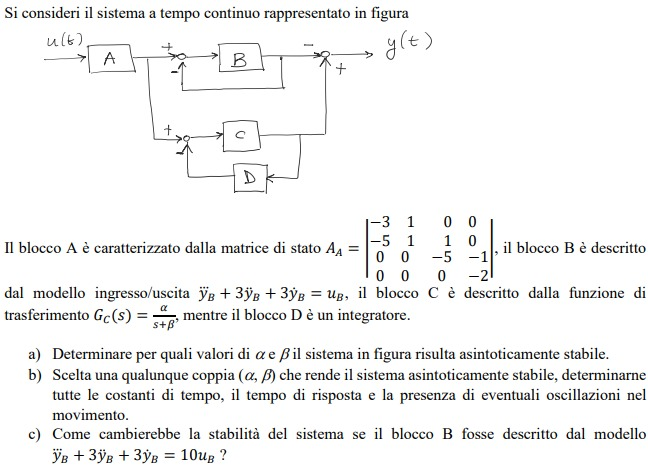
\includegraphics[width=\textwidth]{seconda_domanda}
\end{figure}
\underline{Risposte:}
\begin{enumerate}[a)]
\item Notiamo che questo sistema non è altro che il sistema A in serie al parallelo di due retroazioni negative ($\retroneg$). Dunque per scoprire la stabilità del sistema dobbiamo provare che i sistemi A, $B\retroneg 1$, $C \retroneg D$ sono tutti stabili. 

\begin{itemize}
\item Partiamo da A. Ora, il problema ci dice che:
\[
A_A=\begin{bmatrix}
-3 & 1& 0& 0\\
-5& 1& 1& 0\\
0& 0& -5& -1\\
0 & 0 & 0& -2
\end{bmatrix}
\]
Notiamo che la matrice $A_A$ è triangolare alta a blocchi con:
\[
A_1=\begin{bmatrix}
-3& 1\\
-5& 1
\end{bmatrix} \text{ e } A_2=\begin{bmatrix}
-5& -1\\
0& -2
\end{bmatrix}
\]
Poichè $A_2$ stessa è triangolare alta è immediato vedere che $\lambda_1=-5$  e  $\lambda_2=-2$. Per $A_1$ invece risolviamo il polinomio caratteristico:
\[
\lambda^2+2\lambda+2\longrightarrow \lambda_{1,2}=-1\pm i
\]
Quindi gli autovalori della matrice $A_A$ sono $\{\lambda\}_{A}=\{-5,-2,-1+i,-1-i\}$ e poichè $\Re(\lambda_i)\leq0\quad\forall i$ il sistema è \textbf{Asintoticamente Stabile}

\item Passiamo ora al sistema  $B\retroneg 1$, il problema ci dice che:
\[
\dddot{y}_B+3\ddot{y}_B+3\dot{y}_B=u_B\xrightarrow[]{\,\text{ passando per il polinomio in s }\,}  G_B(s)=\frac{1}{s^3+3s^2+3s}
\]
Per le proprietà dei sistemi a retroazione negativa:
\begin{align*}
G_{(B\retroneg 1)}(s)=&\frac{G_B(s)}{1+G_B(s)}=\frac{1}{s^3+3s^2+3s}\cdot\frac{1}{1+\frac{1}{s^3+3s^2+3s}}=\\
=&\frac{1}{\cancel{s^3+3s^2+3s}}\cdot \frac{\cancel{s^3+3s^2+3s}}{s^3+3s^2+3s+1}=\boxed{\frac{1}{s^3+3s^2+3s+1}}
\end{align*}
Ora ci è facile vedere che il numeratore non è nient'altro che un cubo di binomio:
\[
G_{(B\retroneg 1)}(s)=\frac{1}{s^3+3s^2+3s+1}=\frac{1}{(s+1)^3}
\]
Da ciò deduciamo che $\{\lambda\}_{\left(B\retroneg 1\right)}=\{-1\}$ con molteplictà $3$. Visto che $\Re(-1)<0$ il sistema è  \textbf{Asintoticamente stabile}.
\item Infine analiziamo il sistema $C\retroneg D$, il problema ci dice:
\[
G_C(s)=\frac{\alpha}{s+\beta}
\]
e che D è un intregatore $(\dot{y}=u)$ ossia che:
\[
G_D(s)=\frac{1}{s}
\]
sempre per le proprietà della retroazione negativa:
\begin{align*}
G_{C\retroneg D}(s) &= \frac{G_C(s)}{1+G_C(s)\cdot G_D(s)} = \frac{\alpha}{s+\beta} \cdot \frac{1}{1+\frac{1}{s} \cdot \frac{\alpha}{s+\beta} }\\
&=\frac{\alpha}{s+\beta}\cdot \frac{s^2+\beta}{s^2+\beta s+\alpha}=\frac{\alpha}{\cancel{s+\beta}} \cdot \frac{s\cancel{(s+\beta)}}{s^2+\beta s+\alpha}\\
&=\boxed{\frac{\alpha s}{s^2+\beta s+\alpha}}
\end{align*}
data questa funzione di trasferimento usiamo il criterio di traccia e determinante per sistemi lineari a tempo continuo, con $\det(A)=\alpha$ e  $\tr(A)=-\beta$
\[
\boxed{A.S.}\iff\left\{\begin{array}{l}
\tr(A)<0\\
\det(A)>0
\end{array}\right.\iff\left\{\begin{array}{l}
-\beta<0=\beta>0\\
\alpha>0
\end{array}\right.
\]
Dunque poichè il sistema $S=A\cdot((B\retroneg 1)\parallelsum(C\retroneg D))$ ha come autovalori l'unione di tutti gli autovalori dei sistemi che lo compongono e poichè ognuno di questi sistemi (premesso che $\alpha>0$ e $\beta>0$) è \textbf{Asintoticamente stabile} allora anche S lo è.
\end{itemize}
\item Poichè ci vengono chieste le costanti di tempo e queste sono legate agli autovalori dalla relazione $T_i=-\frac{1}{\Re(\lambda_i)}$ dobbiamo calcolarci questi ultimi. Come detto al punto a):
\[
\{\lambda\}_S=\{\lambda\}_A\cup\{\lambda\}_{B\retroneg 1}\cup\{\lambda\}_{C\retroneg D}
\]
Ora, conosciamo già gli autovalori di A ($\{-5,-2,-1+i,-1-i\}$) e di $C\retroneg D$ ($\{-1\}$), ci restano quindi da determinare gli autovalori di $B\retroneg 1$, scegliamo $\alpha=1$ e $\beta=2$, se operiamo questa scelta:
\[
G_{B\retroneg 1}=\frac{s}{s^2+2s+1}=\frac{s}{(s+1)^2}\implies\lambda_{1,2}=-1\text{ con molteplicità doppia}
\]
Dunque gli autovalori saranno $\{\lambda\}_S=\{-1+i,-1-i,-1,-5,-2\}$ e i tempi di risposta saranno quindi $\{T\}_S=\{\frac{1}{5},\frac{1}{2},1\}$, notiamo che il tempo di risposta $T=1$ è associato a più sottosistemi (e più autovalori) ed è anche la costante di tempo dominante $T_D=1$, da cio deduciamo che:
\[
T_R=5\cdot T_D=5
\]
Inoltre poichè nel sistema sono presenti due autovalori complessi saranno anche \textbf{presenti delle oscillazioni}.
\item Se la funzione di trasferimento di B diventa $G_B(s)=\frac{10}{s^3+3s^2+3s}$ la funzione di trasferimento di $B\retroneg 1$ diventa:
\[
G_{B\retroneg 1}(s)= \frac{10}{s^3+3s^2+3s} \cdot \frac{1}{1+\frac{10}{s^3+3s^2+3s}} = \frac{10}{\cancel{s^3+3s^2+3s}}\cdot \frac{\cancel{s^3+3s^2+3s}}{s^3+3s^2+3s+10}
\]
\smallskip


Dunque data $G_{B\retroneg 1}(s)=\frac{10}{s^3+3s^2+3s+10}$ utiliziamo il criterio di Hurwitz per matrici $3\times 3$
\smallskip
con $\alpha_1=3,\alpha_2=3,\alpha_3=10$, infatti:
\[
\left\{\begin{array}{l}
\alpha_1=3>0\\
\alpha_2=3>0\\
\alpha_3=10>0\\
\alpha_1\alpha_2>\alpha_3=9>10 \text{ che è falso }
\end{array}\right.
\]
Dunque possiamo affermare che non esistono autovalori con parte reale strettamente negativa (quindi il sistema non è \textbf{Asintoticamente Stabile}), dobbiamo provare che non esistono autovalori con $\Re(\lambda)=0$ che soddisfano il polinomio caratteristico di $B \retroneg 1$ cioè che il sistema non è nemmeno \textbf{Semplicemente Stabile}. 
\medskip

Ora, poichè $P(0)_A=10\neq 0$, l'autovalore che cerchiamo (se esiste) è della forma $\pm i\omega$ e:
\[
\text{ per } i\omega\text{ otteniamo }\longrightarrow-i\omega^3-3\omega^2+3i\omega+10=0
\]
Da cui otteniamo il sistema:
\[
\left\{\begin{array}{l}
-\omega^3+3\omega=0\\
-3\omega^2+10=0
\end{array}\right.
\]
Che non ha soluzione, dunque il sistema è \textbf{Instabile}.
\end{enumerate}
\subsection*{Quesito 3}
\underline{Risposte:}
\begin{enumerate}[label= Domanda \arabic*)]
\item risposta 3
\item risposta 2
\item risposta 2
\item risposta 4
\item risposta 3, la perdita di grado è dovuta al fatto  che il sistema è proprio $(d=0)$.
\end{enumerate}
\subsection*{Quesito 4}
\begin{figure}[h]
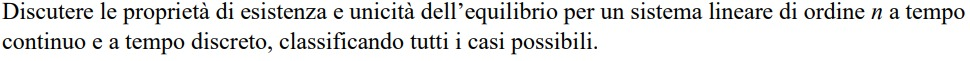
\includegraphics[width=\textwidth]{quarta_domanda}
\end{figure}
\subsubsection{Tempo continuo:}
\underline{Esistenza e Unicità:}\newline
\bigskip
Se esiste l'equilibrio esiste allora $x(t)=\overline{x}\quad\forall t\implies\frac{dx}{dt}=\dot{x}=0\quad\forall t$ e $\dot{x}=Ax+bu\xrightarrow[]{\,\text{ equilibrio }\,}A\overline{x}+b\overline{u}=0$ che ci da n equazioni in n incognite, dunque per il teorema di Rouchè-Capelli:
\begin{itemize}
\item $\exists A^{-1} \iff \det(A)\neq0 \iff \nexists \lambda=0\iff \exists! \overline{x}=-A^{-1}b\overline{u}$
\item $\nexists A^{-1} \iff \det(A)=0 \iff \exists \lambda=0\iff$ fissato $\overline{u}$ allora: $\left\{\begin{array}{l}
\nexists \overline{x}\\
\exists_\infty \overline{x}
\end{array}\right.$
\end{itemize}
\underline{Classificazione Equilibri:}
\begin{itemize}
\item $\Re(\lambda_i)<0 \forall i\iff A.S.$
\item $\exists j/\Re(\lambda_i)>0\implies$ I (forte o esponenziale)
\item $\Re(\lambda_i)\leq 0 \forall i, \exists j:\Re(\lambda_i)=0$ \begin{enumerate}
\item $b_j=1$ ($\lambda_j$ è una radice semplice di $\psi_A$)$\iff$ S.S.
\item $b_j>1$ ($\lambda_j$ è una radice multipla di $\psi_A$)$\iff$ I (debole o polinomiale)
\end{enumerate}
\end{itemize}
\subsubsection{Tempo discreto:}
\underline{Esistenza e Unicità:}\newline
\smallskip
$\exists!\overline{x}$ tale che $x(t+1)=Ax(t)+bu(t)$ e $u(t9=\overline{u}, \quad x(t)=\overline{x}\quad\forall t$ e $x(t+1)=x(t)=\overline{x}$ e il sistema $\overline{x}=A\overline{x}+b\overline{u}$ ci dà n equazioni in n incognite e se lo modifichiamo $(I-A)\overline{x}=b\overline{u}$, dunque sempre il teorema di Rouchè-Capelli:
\begin{itemize}
\item $\exists(I-A)^{-1}\iff\det(I-A)\neq0\iff\text{ A non ha autovalori in 1}\iff \exists!\overline{x}=(I-A)^{-1}b\overline{u}$
\item $\nexists (I-A)^{-1}\iff\det(I-A)=0\iff\text{ A ha almeno autovalore in 1}\iff\left\{\begin{array}{l}
\nexists \overline{x}\\
\exists_\infty \overline{x}
\end{array}\right.$
\end{itemize}
\underline{Classificazione Equilibri:}
\begin{itemize}
\item $|\lambda_i|<1 \forall i\iff A.S.$
\item $\exists j/|\lambda_i|>1\implies$ I (forte)
\item $|\lambda_i|\leq 1 \forall i, \exists j:|\lambda_i|=1$ \begin{enumerate}
\item $b_j=1\quad \forall j/|\lambda_j|=1$ ($\lambda_j$ è una radice semplice di $\psi_A$)$\iff$ S.S.
\item $b_j\neq 1$ ($\lambda_j$ è una radice multipla di $\psi_A$)$\iff$ I (debole o polinomiale)
\end{enumerate}
\end{itemize}

\end{document}
